% !TEX program = lualatex
% !TEX encoding = UTF-8 Unicode
% !TEX spellcheck = de_DE
% 
% Vorlage für Bachelorarbeiten
% 
% Um die Vorlage mit LaTeX zu erstellen sind folgende Programme aufzurufen:
% > lualatex hauptdatei.tex
% > biber hauptdatei
% > lualatex hauptdatei.tex

\documentclass{scrbook}

% !TEX root = hauptdatei.tex
% !TEX encoding = UTF-8 Unicode
% !TEX spellcheck = de_DE
%
% für mehr Informationen zu einzelnen Paketen siehe zum Beispiel:
% http://texdoc.org/pkg/paketname
% http://ctan.org/pkg/paketname


%% Setzen von Dokumentenoptionen:
%% (aquivalent zu \documentclass[<Optionen>]{...}

%%% Layout-Einstellungen
	\KOMAoptions{ 				% aquivalent zu \documentclass[<Optionen>]{...}
		fontsize=12pt,			% Standartschriftgröße
		bibliography=totoc,	% Bibliografie soll im Inhaltsverzeichnis auftauchen
		headings=normal,		% Größe und Abstand von Überschriften
		toc=listof,				% Verzeichnisse der Gleitumgebungen ins Inhaltsverz.
		toc=indent,				% Inhaltsverzeichnis in hierarchischer Form
		listof=indent,			% andere Verzeichnisse in hierarchischer Form
		listof=totoc,           % andere verzeichnisse im Inhaltsverzeichnis führen
		twoside=false				% enseitiges Layout
	}
	\setcounter{tocdepth}{1} % Ebenentiefe des Inhaltsverzeichnis
	\usepackage{geometry, setspace}
	\geometry{
		paper=a4paper,		% DIN A4 Papier
		hmargin=30mm,			% horizontale Seitenränder
		top=15mm,				% oberer Rand
		bottom=20mm,			% unterer Rand
		includeheadfoot,	% Kopf- und Fußzeilen gehören nicht zum Rand
	}
	\onehalfspacing 		% anderthalbfacher Zeilenabstand
	% Kapitelüberschrift etwas nach oben versetzen:
	\renewcommand*{\chapterheadstartvskip}{\vspace*{-1.48\topskip}}


%% Einstellung der Schriftart:
	\usepackage{lmodern}
	% Alternativ können mit fontspec beliebige im Betriebssystem installierte Schriften verwendet werden:
	%\usepackage{fontspec}
	%\setmainfont{Constantia}
	%\setsansfont{Corbel}
	%\setmonofont{Consolas}
	% Für Serifen in den Überschriften:
	%\addtokomafont{sectioning}{\rmfamily}


%% Einstelen von Kopf- und Fußzeilen:
	\usepackage[headsepline=false]{scrlayer-scrpage}
	% automatisches Füllen der Kopfzeile mit aktuellem Kapitel/Abschnitt:
	\automark[chapter]{chapter}
	% links, mitte, rechts
	\lohead{}
	\cohead{}
	\rohead{}
	% Seitenzahl nur auf plain-Seiten im Fuß
	\lofoot{}
	\cofoot*{\pagemark}
	\rofoot{}
	% Aktivieren des festgelegten Kopfzeile:
	\pagestyle{scrheadings}


%% Sprachauswahl:
	\usepackage{polyglossia}
	\setmainlanguage{english}
	% die Sprache kann im Dokument mit
	% \begin{english} ... \end{english}
	% umgestellt werden


%% Einstellungen zu Zitaten und Bibliografie:
\usepackage{csquotes}

\usepackage[
backend=biber,
bibstyle=apa,
citestyle=apa,
]{biblatex}
\addbibresource{thesis.bib}


\setlength{\bibhang}{15pt}
\defbibenvironment{bibliography}
  {\list
     {}
     {\setlength{\leftmargin}{\bibhang}%
      \setlength{\itemindent}{-\leftmargin}%
      \setlength{\itemsep}{\bibitemsep}%
      \setlength{\parsep}{\bibparsep}}}
  {\endlist}
  {\item}
  \addspace

\setlength\bibitemsep{1.3\itemsep}


	%% sonstige Pakete:
	\usepackage{
		array,		% erweiterte Option für Tabellen
		booktabs,	% schöne Tabellen
		float,		% Platzierung von Gleitobjekten (Abb., Tab.), Eigene Gleitobjekte
		graphicx,	% ermöglicht einbinden von Grafiken mit \includegraphics
		hologo,		% für TeX-Logos
		mathtools,	% Verbesserungen für den Mathesatz (läd u.a. amsmath)
		microtype,	% mikrotypografische Verbesserungen (z.B. optischer Randausgleich)
		paralist,	% platzsparende Listen mit compactitem
		xcolor,		% Verwendung von Farbe
	}


%% LaTeX sucht nach Bildern an den hier angegebenen Stellen:
	\graphicspath{{./images/},{./}}


%% automatische PDF-Verlinkungen im Dokument:
	\usepackage[
		colorlinks=false,		% Links nicht farbig hervorheben
		pdfborder={0 0 0},		% links nicht durch PDF-Kasten hervorheben
	]{hyperref}






\addbibresource{thesis.bib}


\usepackage{tikz}

\usepackage{array,makecell}
\usepackage[format=plain, labelfont=bf]{caption}


\usepackage{tabularx}
    \renewcommand\tabularxcolumn[1]{m{#1}}
    \newcolumntype{C}{>{\centering\arraybackslash}X}

\newcommand{\ExternalLink}{%
    \tikz[x=1.2ex, y=1.2ex, baseline=-0.05ex]{% 
        \begin{scope}[x=1ex, y=1ex]
            \clip (-0.1,-0.1) 
                --++ (-0, 1.2) 
                --++ (0.6, 0) 
                --++ (0, -0.6) 
                --++ (0.6, 0) 
                --++ (0, -1);
            \path[draw, 
                line width = 0.5, 
                rounded corners=0.5] 
                (0,0) rectangle (1,1);
        \end{scope}
        \path[draw, line width = 0.5] (0.5, 0.5) 
            -- (1, 1);
        \path[draw, line width = 0.5] (0.6, 1) 
            -- (1, 1) -- (1, 0.6);
        }
    }


\usepackage{booktabs, caption, makecell}
\renewcommand\theadfont{\bfseries}
\usepackage{threeparttable}

\counterwithout{footnote}{chapter}


%% Alle wichtigen Einstellungen sind in der Datei einstellungen.tex getätigt
%% und können dort verändert werden.

\begin{document}
	
\frontmatter
\begin{titlepage}

\begin{center}

\vspace*{1,2cm}

\huge {\bfseries The impact of vaccine lotteries on COVID-19 vaccination
rates: Evidence from Poland}\\[1.8cm]

\Large {Bachelor Thesis}\\[1cm]

\large {Department of Economics}\\[0.2cm]

\large {University of Mannheim}\\[0.5cm]

\end{center}

\vfill

\noindent submitted to:\\
Prof.~Achim Wambach, PhD / Sabrina Schubert\\[1cm]
submitted by:\\
Benedikt Stelter\\[1cm]
Student ID: 1731015\\
Degree Program: Bachelor of Science in Economics (B.Sc.)\\[1cm]
Address: Meerfeldstr. 11, 68163 Mannheim\\
Phone: +49 176 95741248\\
E-Mail: benedikt.stelter@students.uni-mannheim.de\\[1cm]
Mannheim, 17/03/2023

\setcounter{page}{0}

\end{titlepage}

  \tableofcontents


%% Abbildungsverzeichnis
\listoffigures

%% Tabellenverzeichnis
\listoftables


\mainmatter

\chapter{Introduction}

In March 2020, the world came to a sudden stop due to the spread of
COVID-19. Governments took drastic and unprecedented steps to slow the
spread of the virus: Shops were shut down, schools and universities were
closed and millions of workers had to work from their home office or
kitchen desk.

Just a year after the first cases appeared in China, the first vaccines
against COVID-19 were approved for emergency use
\parencite{us_food_and_drug_administration_fda_2020}. With them came the
hope of a return to normality and a severe reduction of the pandemic's
death toll. At the beginning of the vaccination effort in Europe, the
supply of vaccines was not able to meet the demand at the necessary
speed and scale \parencite{bongardt_europes_2021}. Therefore, a shortage
of vaccines lead to rationing: Vaccines were only provided to the most
vulnerable groups of the population, such as healthcare workers or the
elderly. When vaccines became widely available, policymakers had to
learn that a considerable share of people were hesitant or unwilling to
receive the vaccine \parencite{steinert_covid-19_2022}. Globally, the
COVID-19 vaccine was one of the most relevant and hotly contested topics
of 2021, demonstrated by Google
Trends\footnote{see \url{https://trends.google.de/trends/yis/2021/GLOBAL/} (Retrieved March 7, 2023).},
which placed the COVID vaccine as the third most searched news story of
the entire year of 2021.

To increase vaccine uptake, some governments decided to offer various
sorts of incentives to get vaccinated \parencite{wyllie_jewellery_2021}.
One of these incentives were vaccine lotteries. A vaccine lottery, in
the context of this thesis, refers to a lottery with cash or non-cash
prizes, in which only vaccinated people could participate, thereby
acting as a possible reward for vaccination. Policymakers hoped that
this would persuade additional people to get vaccinated, increasing the
total vaccination rate of the population.

Several lotteries of this sort have been carried out around the world,
whose effects have been widely investigated. For example, studies
suggest that most but not all of the state lottery programs implemented
in the US were successful in increasing vaccine uptake
(\cite{robertson_are_2021}; \cite{acharya_implementation_2021};
\cite{fuller_assessing_2022}). Three vaccine lotteries have been
implemented in Europe: In Romania, Slovakia and Poland. Poland was the
first European country to implement such a policy and offers good
preconditions (data availability, detailed information about the
lottery) to investigate the effectiveness of vaccine lotteries in
Europe. This thesis therefore tries to answer the question: What are the
effects of vaccine lotteries on the share of the population vaccinated
against COVID-19?

In order to spur the national vaccination campaign, the Polish
government announced the lottery
\parencite{service_of_the_republic_of_poland_national_2021} on May 25,
2021, around five months after the authorization of the first COVID-19
vaccines in the EU and the subsequent start of the Polish vaccination
campaign. It was open from July 1, 2021 until September 30, 2021. The
main prize of the lottery was a cash prize of one million zł
(zloty)\footnote{At the time of announcement on 25/05/2021, one million zł were equal to around 220,000 €, at an exchange rate of 0.22 zł to €.},
but it also included smaller cash and non-cash prizes and a lottery-like
incentive scheme for municipalities.

Among with other vaccination incentives in Europe,
\textcite{kuznetsova_effectiveness_2022} shortly evaluated the effects
of this lottery on daily vaccinations using a time-series model,
suggesting a positive effect of the policy. To this day, there has
however been no study evaluating the Polish vaccine lottery in detail.
This thesis therefore adds a new case study to the existing literature
on the effects of COVID-19 vaccine lotteries.

The quasi-experimental empirical analysis consists of two parts. To
begin with, a regression discontinuity design is employed to evaluate
the effect of the lottery on daily vaccinations, similar to the analysis
by \textcite{kuznetsova_effectiveness_2022}. The main analysis is
conducted using the synthetic control method based on
\textcite{abadie_economic_2003}, a popular method for comparative case
studies. The basic idea of the synthetic control method is to create a
synthetic control unit as a combination of multiple control units (donor
pool), to then estimate the treatment effect of a policy/intervention.
Out of a donor pool of six other Eastern European countries and using
additional predictor variables, a synthetic control unit (``Synthetic
Poland'') is constructed to evaluate the effect of the policy on
vaccination rates of both the fully vaccinated as well as the share of
the population with at least one dose. Data on daily vaccinations and
vaccination rates, published by the respective governments/government
agencies and collected by Our World in Data
\parencite{mathieu_global_2021}, as well as additional data from
\textcite{eurostat_eurostat_2023} and the Wellcome Global Monitor, also
collected by \textcite{our_world_in_data_share_2020}, are exploited for
the analysis.

The empirical analysis finds no evidence for a significant increase in
the share of the population fully vaccinated against COVID-19 as a
result of the lottery, with an estimated effect of one percentage point.
Similarly, a significant effect on daily vaccinations is not found.
While the synthetic control estimation does not show to be very robust,
the analysis suggests that the lottery might have incentivized some
people who would have gotten vaccinated anyway to do this earlier, in
order to take advantage of the lottery, thereby potentially increasing
the vaccination rate (fully vaccinated) temporarily by around five
percentage points.

The thesis is structured as follows: Chapter 2 provides background
information about the existing literature and the policy. Chapter 3
discusses the methodology and the data used for the empirical analysis.
The results are presented in Chapter 4 and discussed in Chapter 5.

\chapter{Background}

\section{Literature review}

\subsection*{Policies to influence individual health behaviors}

Tobacco and alcohol consumption, obesity, viral diseases: Governments
are facing many challenges from a public health perspective. Behavioral
economics can offer several ways to influence the decisions of
individuals, in order to encourage (socially) desirable behavior. The
least severe tool to influence individual health decisions might be
nudges.

Nudging is a concept mainly brought to the public through the work of
\textcite{thaler_nudge_2008}. The authors define a nudge as an
intervention that ``alters people's behavior in a predictable way
without forbidding any options or significantly changing their economic
incentives'' (p.~6). Nudging can be applied in various ways, but it is
often connected to health lifestyle topics, such as nutrition and diet
\parencite{ledderer_nudging_2020}. For example, in an experiment in
Denmark \parencite{friis_comparison_2017}, the objective was to promote
the consumption of vegetables in the setting of a self-serving buffet,
which included salads and other dishes in large bowls. As a nudge, the
food environment was changed by arranging green plants and herbs around
the food bowls. In a second experiment, salad was pre-portioned into
smaller take-away bowls. The results showed that the intake of energy
from vegetables of the participants can be increased by pre-portioning
the salad. Although many studies evaluating the impact of nudges suggest
positive effects of the respective interventions, these results should
be interpreted with caution, since a lot of studies, including
\textcite{friis_comparison_2017}, were conducted in the lab and may
therefore not be reproducible in a real-world setting
\parencite{ledderer_nudging_2020}.

Besides nudging, policymakers could significantly change economic
incentives. This has especially been applied in drug policy, for example
to reduce alcohol and tobacco consumption. Both in developed and
developing countries, it has been shown that raising prices (through
higher taxation) can lead to reduced consumption of tobacco
(\cite{yeh_effects_2017}; \cite{immurana_effects_2021}) as well as
alcohol \parencite{daley_impact_2012}.

Beyond taxation, governments might also use other financial incentives
to motivate changes in individual behavior, such as (small) cash
payments or lotteries. Several meta-analyses found that such incentives
can be successful in inducing behavior changes at the individual level.
For example, \textcite{giles_effectiveness_2014} evaluated 16 studies on
issues such as smoking cessation, health screenings, physical activity
and vaccinations. The authors found that financial incentives are
effective at encouraging healthy behavior. This finding was also
confirmed by \textcite{mantzari_personal_2015}, who evaluated 34 studies
and additionally concluded that this effect is stronger for the most
deprived individuals, thereby possibly reducing health inequalities.
Lotteries have also been shown to be effective in certain public health
settings. \textcite{bjorkman_nyqvist_incentivizing_2018} found that the
introduction of a lottery program reduced HIV incidence in Lesotho.
Lotteries also increased cycling \parencite{ciccone_using_2021} and
walking activity \parencite{patel_randomized_2018} as well as
participation in chlamydia screenings \parencite{niza_vouchers_2014}
under specific settings.

\subsection*{Policies to increase COVID-19 vaccine uptake}

When a considerable degree of citizens were unwilling to get vaccinated
in Europe \parencite{steinert_covid-19_2022}, governments thought about
ways to encourage their citizens to get vaccinated, using incentives as
well as other measures.

One widely used tool were vaccine passports (e.g.~in Europe
\parencite{niestadt_domestic_2021}). Access to social gatherings (such
as restaurants, bars, clubs, stadiums), international travel and
quarantine regulations were made subject to certified vaccination
against COVID-19. Besides ethical concerns, for example potential
disqualification of minorities from social life
\parencite{gostin_digital_2021}, the evidence on the effectiveness of
such regulations is mixed. A synthetic control analysis of six countries
found that COVID passports were successful in increasing daily
vaccinations in countries with lower than average vaccination rates. In
other countries, these regulations were less effective
\parencite{mills_effect_2022}. In Eastern Europe, a comparison between
Poland (very restricted use of COVID passports) and Lithuania (wide use
of COVID passports) suggested a positive effect on vaccination rates
\parencite{walkowiak_covid-19_2021}. It should be noted that COVID
passports may have even had negative effects on vaccine uptake, since
frustration about reduced autonomy might have lowered willingness to get
vaccinated \parencite{porat_vaccine_2021}.

Besides the carrot-and-stick approach, governments also used nudges and
economic incentives, such as cash payments and non-cash rewards, to
increase COVID-19 vaccination rates. Using a randomized control trial,
\textcite{campos-mercade_monetary_2021} found that even ``small'' cash
payments of around 24 \$ could significantly increase vaccination rates,
while small nudges, such as information about the safety and
effectiveness of the vaccine, were not successful. While some studies
have also suggested a measurable positive effect of cash payments on
vaccination rates (\cite{wong_guaranteed_2022};
\cite{kluver_incentives_2021}; \cite{kim_vaccination_2021-1}), there is
also evidence against their effectiveness. \textcite{jacobson_can_2022}
suggested that neither behavioral nudges (reminder to get vaccinated via
text message) nor cash payments could increase vaccination rates among
the hesitant citizens. \textcite{sprengholz_money_2021} also found that
cash incentives did not increase willingness to get vaccinated.

A specific version of economic incentives are lotteries.
\textcite{dube_exploring_2022} analysed the effectiveness of a vaccine
lottery in Québec (Canada) and found a small positive impact on
vaccination intentions. A survey, conducted by
\textcite{jun_association_2022}, concluded that a vaccine lottery in
Australia successfully increased willingness to get vaccinated. Most
evidence on the effectiveness of vaccine lotteries deals with state
vaccine lotteries in the US. For example, studies on vaccine lotteries
in Louisiana and Massachusetts found different effects. Whereas the
lottery in Louisiana increased vaccine uptake
\parencite{wang_moving_2023}, a vaccine lottery in Massachusetts did not
significantly increase vaccination rates, although prizes were higher
\parencite{kim_did_2023}.

A specific focus can be observed with respect to Ohio. There are several
studies evaluating the Ohio Vax-A-Million lottery
\parencite{ohio_department_of_health_ohio_2021}, which was one of the
first COVID-19 vaccine lotteries in the US. In total, a majority of the
reviewed literature has cast a positive light on the efficacy of the
lottery. So far, there have been four studies evaluating the lottery
using the synthetic control method. These studies constructed Synthetic
Ohio out of a donor pool of other US states. Three of these four studies
have found small positive effects of the lottery on vaccine uptake
(\cite{brehm_ohio_2022}; \cite{barber_conditional_2022};
\cite{sehgal_impact_2021}) and one did not find a significant effect
\parencite{lang_did_2022}. Using other methods,
\textcite{mallow_covid-19_2022} also found a positive effect of the
lottery on vaccination rates, while \textcite{walkey_lottery-based_2021}
did not find such an effect.

\section{Institutional background}

The Polish vaccination campaign started on December 27, 2020, when a
nurse from a Warsaw Hospital received the first vaccine dose
\parencite{waligora_how_2021}. Citizens who wanted to get vaccinated had
to register and select their preferred vaccine prior to vaccination. In
May 2021, the waiting time between the first and the second dose
(Janssen (Johnson \& Johnson) required only one dose) was set at five
weeks \parencite{service_of_the_republic_of_poland_changes_2021}. In the
first weeks and months of the vaccination campaign, vaccines were only
available to health care workers and senior citizens. By the start of
May 2021, vaccines became widely available
\parencite{koschalka_poland_2021}.

In general, vaccination rates in Poland have been low compared to the
rest of the EU, with the Polish vaccination rate at around 50\% by the
end of September 2021, compared to an EU average of more than 60\%. In
the context of Eastern Europe, vaccination rates have been relatively
close to the average. Many Eastern European countries experienced
relatively low vaccination rates \parencite{mathieu_global_2021}. In the
media, a general distrust in the government and a lack of educational
campaigns \parencite{vaccines_today_polands_2021} as well as chaotic and
conflicting communication by government officials
\parencite{wanat_polands_2021} have been cited as potential reasons for
the low vaccine uptake in Poland.

\renewcommand*{\arraystretch}{1.5}
\begin{table}[! htbp]\centering \caption[Prizes of Polish lottery]{The Polish vaccine lottery consisted of four types of draws and included cash and non-cash prizes.}
\bigskip
\label{table:summarystat}
\begin{threeparttable}
\begin{tabularx}{10.5cm}{c|c|c}
\toprule
 & \thead{Cash prizes} & \thead{Non-cash prizes}\\ \midrule
Instant & \(13,000*500\) zł & - \\
 & \(39,000*200\) zł & \\ \hline
Weekly & \(60*50,000\) zł & 720 electric scooters \\  \hline
Monthly & \(6*100,000\) zł & 6 small vehicles \\ \hline
Main & \(2*1,000,000\) zł & 6 middle class vehicles \\
\bottomrule
\end{tabularx}
\begin{tablenotes}
      \item \footnotesize Source: \textcite{service_of_the_republic_of_poland_national_2021}
    \end{tablenotes}\end{threeparttable}
\label{table2}
\end{table}

\renewcommand*{\arraystretch}{1}

To increase vaccination rates, Poland decided to implement a vaccine
lottery. The lottery, which is investigated empirically in this thesis,
was open from July 1, 2021 to September 30, 2021. It was announced on
May 25, 2021 \parencite{charlish_poland_2021}. The policy had two main
elements: A lottery for all adult fully vaccinated people (two doses)
\parencite{service_of_the_republic_of_poland_national_2021} and a
monetary incentive scheme for municipalities
\parencite{service_of_the_republic_of_poland_competitions_2021}. The
main prize of the lottery was a cash prize of one million zł (awarded
twice), but it also included smaller monthly, weekly and daily cash
prizes along with non-cash prizes (cars and electric scooters),
amounting to a total cost of roughly 140 million zł
\parencite{wilczek_poland_2021}. A detailed overview of the lottery is
depicted in Table 2.1. Citizens were able to enter the lottery both
online and by phone. It was organized by the state-owned polish lottery
company Totalizator Sportowy, which also operates other popular
lotteries in Poland. Poland's lottery can be seen as a mixture of
different types of lotteries. Especially in the US, state governments
have focused on lotteries with high rewards and relatively low winning
probabilities
(e.g.~Ohio\footnote{see \textcite{ohio_department_of_health_ohio_2021}.},
Massachusetts\footnote{see \textcite{commonwealth_of_massachusetts_massachusetts_2021}.}
with prizes of one million \$). Another possibility could be the use of
relatively low prizes (e.g.~below 1000 \$) with higher winning
probabilities. The Polish policy included relatively small prizes
(instant prizes) but also larger prizes (main draw), thereby combining
both elements. The vaccine lottery to be considered as the most similar
to Poland's is the one implemented in Romania, in October 2021
(announced in September), which also included a similar mixture of
larger and smaller prizes
\parencite{health_ministry_of_romania_press_2021}.

As part of the monetary incentive scheme for municipalities, the
municipality with the highest percentage of the vaccinated in the
country received two million zł. Three other municipalities who had the
highest percentage of the vaccinated in their respective comparison
group\footnote{There were three groups: Municipalities with a population of up to 30,000 people, cities with a population of 30,000 - 100,000 and large cities with a population above 100,000.}
received one million zł each. 500 other municipalities, who were among
the fastest in the country to reach a vaccination rate of 67\%, won
100,000 zł each.

\chapter{Data and methodology}

\section{Data}

The main data for the empirical analysis was taken from a data set
created by Our World in
Data\footnote{As of March 8, 2023. Link to GitHub repository: \url{https://github.com/owid/covid-19-data/tree/bac6f96045857196fa439508492529d5b9e75d0e}.}
\parencite{mathieu_global_2021}. This data set is a collection of the
number of daily vaccinations, vaccination rates as well as other
vaccination-related indicators from all countries of the world, coming
directly from the respective governments/government agencies and
collected by Our World in Data. If provided by the governments, the data
set offers a daily time series of the described indicators.

For most of the donor pool countries however, several observations were
missing. Linear interpolation was used to replace the missing
observations, by drawing a straight line between the two adjacent data
points. Other imputation techniques were also considered. Some of these,
such as last observation carried forward (LOCF) or mean imputation, did
not seem attractive in the given setting, since the vaccination rate is
a monotonically increasing function.

For the synthetic control analysis, additional predictor variables were
used (the choice of these variables is explained in Section 3.4). The
data for these variables was extracted from
\textcite{eurostat_eurostat_2023} as well as from a survey by the
Wellcome Global Monitor, also collected by
\textcite{our_world_in_data_share_2020}.

\section{Regression discontinuity design}

Regression discontinuity design is a method to estimate treatment
effects in settings in which the treatment assignment is determined by
whether the running variable \(X_{i}\) exceeds a certain
cutoff/threshold value \(c\). Formally, the treatment status is defined
as: \begin{equation}
D_{i} = \begin{cases}
1 & \text{if}\; X_{i} \geq c \\
0 & \text{if}\; X_{i} < c
\end{cases}
\end{equation} This specific application is an example of a sharp
regression discontinuity design, in which the probability of treatment
changes from 0 to 1 at the cutoff. The discontinuity of the treatment
status around the cutoff allows for an examination of the two sides, by
comparing the limits at the cutoff value. The treatment effect for the
outcome variable \(Y_{i}\) at the cutoff is defined as the difference
between these limits: \begin{align}    
\tau & =\text{E}[Y_{1}-Y_{0}\vert X_{i}=c] \\
     & =\lim_{x\downarrow c} \text{E}[Y_{1}\vert X_{i}=c]-\lim_{x\uparrow c} \text{E}[Y_{0}\vert X_{i}=c] \nonumber
\end{align} \noindent The identifying equation for the estimation, in
which the specific functional form is left open, is given by:
\begin{equation}
Y_{i}=f(X_{i})+\beta D_{i}+\epsilon_{i}
\end{equation} This can also be adjusted to allow for different
functions to the left and to the right of the cutoff: \begin{equation}
Y_{i}=f_{l}(X_{i})I\{X_{i}<c\}+f_{r}(X_{i})I\{X_{i}\geq c\}+\beta D_{i}+\epsilon_{i}
\end{equation} The objective is to estimate \(\beta\), which corresponds
to the local average treatment effect at the cutoff value.

\section{Synthetic control method}

The synthetic control method was first established by
\textcite{abadie_economic_2003}, in order to investigate the economic
effects of terrorism in the basque country, and further developed by
\textcite{abadie_synthetic_2010}.

Synthetic control methodology has been applied widely in economics, but
also in other social sciences such as political science. For instance,
it has been used to evaluate the economic effects of European
integration \parencite{campos_institutional_2019}, the effect of natural
disasters on economic growth \parencite{cavallo_catastrophic_2013} or to
investigate democratic backsliding
\parencite{meyerrose_unintended_2020}. Its area of application are
comparative case studies, in which the comparison of different cases can
allow for conclusions about a certain policy or intervention, which
might be present only in one of the examined cases.

\subsection*{Formal definition}

Researchers want to investigate the effect of a policy or intervention
on a selected variable. The variable of interest is the outcome variable
\(Y_{jt}\) for \(J + 1\) units from \(t=1\) to \(T\). The first unit
(\(j = 1\)) is the treated unit, while all other units are untreated.
The intervention occurs at \(T_{0}+1\), meaning that there are \(T_{0}\)
pre-intervention time periods. There are a total of \(k\) predictors per
unit, which include the pre-intervention observations of the outcome
variable (\(Y_{j1},Y_{j2},...,Y_{jT_{0}}\)) as well as additional time
invariant unit level characteristics \(\mathbf{Z}_{j}\) (as outlined in
Section 3.4). These \(k\) total predictors can be summarized by the
\((k\times 1)\) vectors
\(\mathbf{X}_{j}=(Y_{j1},Y_{j2},...,Y_{jT_{0}},\mathbf{Z}_{j}')'\) for
units \(j=1,...,J + 1\). It is then possible to combine all of the
predictors of the untreated units, in order to obtain the
\((k\times J)\) matrix
\(\mathbf{X}_{0}=(\mathbf{X}_{2},\mathbf{X}_{3},...,\mathbf{X}_{J + 1})\)\footnote{\(\mathbf{X}_0=
\begin{bmatrix}
Y_{21} & Y_{31} & \dots & Y_{J+11}\\
Y_{22} & Y_{32} & \dots & Y_{J+12}\\
\vdots & \vdots & \ddots & \vdots\\
Y_{2T_{0}} & Y_{3T_{0}} & \dots & Y_{J+1T_{0}}\\
\mathbf{Z}_{2}' & \mathbf{Z}_{3}' & \dots & \mathbf{Z}_{J + 1}'
\end{bmatrix}\)}.

The average treatment effect is defined as the difference between the
potential outcome of the treated unit with intervention (\(Y_{1t}^{I}\))
and its potential outcome without the intervention (\(Y_{1t}^{N}\)):
\begin{equation}
\tau_{1t}=Y_{1t}^{I}-Y_{1t}^{N}\; \; \text{for}\; \; t>T_{0}
\end{equation} By definition, the outcome with intervention is known and
the outcome without intervention is hypothetical for the treated unit.
To estimate the treatment effect, it is therefore sufficient to estimate
\(Y_{1t}^{N}\).

The simplest idea to estimate \(Y_{1t}^{N}\) might be to choose the
closest unit \(j^{*}\), the best single control
\parencite{doudchenko_balancing_2016}, as the control unit. This best
single control solves: \begin{equation}
j^{*}=\text{arg}\; \min_{j>1}\vert\vert\mathbf{X}_{j}-\mathbf{X}_{1}\vert\vert
\end{equation} Taking a difference then results in an estimator for the
average treatment effect: \begin{equation}
\hat{\tau}_{1t}=Y_{1t}^{I}-Y_{j^{*}t}\; \; \text{for}\; \; t>T_{0}
\end{equation} However, using a single control approach does not seem
like a desirable estimation method, since it is difficult to achieve a
good fit relative to the treated unit in the pre-treatment period.

The synthetic control method developed by
\textcite{abadie_economic_2003} proposes to use a weighted average of
donor pool units as a synthetic control unit, enabling a better
pre-treatment fit. The synthetic control and the following estimator for
the average treatment effect are defined as: \begin{equation}
\hat{Y}_{1t}^{N}=\sum_{j=2}^{J+1} w_{j}Y_{jt}
\end{equation} \begin{equation}
\hat{\tau}_{1t}=Y_{1t}^{I}-\hat{Y}_{1t}^{N}\; \; \text{for}\; \; t>T_{0}
\end{equation} The weights \(\mathbf{W}=(w_{2},w_{3},...,w_{J+1})'\) are
chosen, such that the synthetic control matches as closely as possible
the pre-intervention path of the predictors of the outcome variable for
the treated unit. Consequently, the weights have to be chosen such that
this difference is minimized. The optimal weights
\(\mathbf{W}^{\star}=(w_{2}^{\star},w_{3}^{\star},...,w_{J+1}^{\star})'\)
solve:

\begin{equation}   
\begin{aligned}
\mathbf{W}^{*}=\text{arg}\; \min \quad & \vert\vert\mathbf{X}_{0}\mathbf{W}-\mathbf{X}_{1}\vert\vert\\
\textrm{s.t.} \quad & w_{j}\in[0,1]\\
  &\sum_{j=2}^{J+1} w_{j}=1   \\
\end{aligned}
\end{equation} The difference is minimized subject to the weights being
non-negative and summing up to one, a crucial assumption in the original
framework proposed by \textcite{abadie_economic_2003}. In several
extensions to this original framework
(e.g.~\textcite{doudchenko_balancing_2016}), this assumption has been
relaxed to allow for negative weights. It is then possible to plug in
the optimal weights \(\mathbf{W}^{\star}\) from the constrained
minimization to obtain the estimated average treatment effect from
(3.9): \begin{equation}
\hat{\tau}_{1t}=Y_{1t}^{I}-\sum_{j=2}^{J+1} w_{j}^{\star}Y_{jt}\; \; \text{for}\; \; t>T_{0}
\end{equation}

\subsection*{Inference}

Based on \textcite{abadie_synthetic_2010} and
\textcite{abadie_using_2021}, the most common way of inference for the
synthetic control method is permutation, through the use of placebo
effects. A synthetic control unit is constructed for all of the
untreated countries in the control group, as if there was a treatment
for these countries (the treated country is then also part of the donor
pool). If the magnitude of the effect for the treated unit is extreme
compared to the placebo synthetic controls of the untreated units, the
effect can be regarded as significant. In order to perform this
analysis, the gaps between the synthetic control and the actual outcome
can be plotted for all selected countries (``placebo plot''), in order
to visually compare the size of the effects. One potential problem of
this concept is the difficulty of obtaining a satisfactory pre-treatment
fit for all units in the donor pool, especially when making use of a
relatively small donor pool. Additionally, inference based on visual
interpretations can be considered as vague, since it does not rely on a
quantitative measure, such as a \textit{p}-value.

A possibility of quantification is to measure the ratio of the
post-intervention fit relative to the pre-intervention fit. First of
all, the root mean squared prediction error (RMSPE) of the synthetic
control is defined: \begin{equation}
R_{j}(t_{1},t_{2}) =(\frac{1}{t_{2}-t_{1}+1}\sum_{t=t_{1}}^{t_{2}}(Y_{jt}-\hat{Y}_{jt}^{N})^2)^\frac{1}{2}
\end{equation} It is then possible to define \(r_{j}\), which measures
the quality of the fit in the post-intervention period compared to
pre-intervention and is given by the ratio of the post-intervention
RMSPE and pre-intervention RMSPE: \begin{equation}
r_{j}=\frac{R_{j}(T_{0}+1,T)}{R_{j}(1,T_{0})}
\end{equation} Using \(r_{j}\), a \textit{p}-value can be computed for
the permuted test: \begin{equation}
p=\frac{1}{J+1}\sum_{j=1}^{J+1}I_{+}(r_{j}-r_{1})
\end{equation}

\subsection*{Requirements}

Several requirements should be fulfilled in order to obtain a valid
synthetic control estimation, outlined by \textcite{abadie_using_2021}.
Firstly, the evaluated policy/intervention should - in principle - be
able to produce a sufficiently large effect. When the effect of an
intervention is too small, it may not be possible to distinguish this
effect from other shocks to the outcome variable. Additionally, the
volatility of the outcome variable should not be too high, to prevent
``over-fitting'', meaning that the synthetic control might react to
certain pre-treatment patterns of the outcome variable which could not
be present post-treatment \parencite{hollingsworth_tactics_2022},
generating a biased estimation.

Secondly, there needs to be a suitable comparison/control group. Units
that are subject to similar interventions or other shocks to the outcome
variable in the given time frame should be excluded from the donor pool.
If this were not done, a negative shock to the outcome variable in one
of the donor pool units could lead to false conclusions. It could be
mistakenly determined that the unit of interest experienced a negative
effect because of the examined intervention, which might only be the
case because of the shock in one of the donor pool units. Furthermore,
researchers should try to select units for the donor pool which are not
too different from the treated unit. Otherwise, it may be difficult to
obtain a good fit of the synthetic control unit before the intervention.

Thirdly, there should be no anticipation effect, meaning that economic
agents do not anticipate the enactment of the respective policy. In
contrast, if agents were to anticipate the intervention before its
actual implementation, the synthetic control analysis could not
successfully estimate the investigated effect. Too many pre-treatment
observations would then be used for the constrained minimization, which
generates the weights of the synthetic control unit.

Next, there should be no spillover effects of the treated unit on
untreated units. If this were the case, the post-treatment values of the
synthetic control unit (which, by definition, consists of untreated
units) would be affected by the treatment, thereby violating the basic
principle of the synthetic control method.

Lastly, regarding the data, it is crucial to have a sufficient number of
pre-treatment observations of the outcome variable, such that a
satisfactory fit of the synthetic control unit can be obtained. A larger
number of pre-intervention outcomes improves the fit of the synthetic
control unit, increasing its robustness and interpretability.

\subsection*{Strengths and weaknesses}

Applying the synthetic control method in comparative case studies offers
several advantages \parencite{abadie_using_2021}. Firstly, the fit of
the synthetic control unit is transparent. A table such as Table 3.1,
which presents the predictors of actual and Synthetic Poland, outlines
the differences between the two units, allowing for a quick evaluation
of whether the use of a synthetic control is appropriate in a specific
application (``are the donor pool units and the treated unit similar
enough?''). Transparency is also an advantage with respect to the
composition of the synthetic control unit. A clear list of the different
weights provides the opportunity to assess the fulfillment of some of
the requirements of the synthetic control, e.g.~the spillover effect.
The problem of a possible spillover effect could be disregarded, if the
country this might apply to has a weight of 0 or very close to 0.
Another advantage might be that only pre-intervention outcomes are used
to construct the synthetic control unit. This could prevent researchers
from changing the specifications of the synthetic control to achieve a
certain result (e.g.~a significant result (\textit{p}-Hacking)), after
initially constructing it. Still, it has to be noted that it is possible
to compare the results of different specifications and select the
specification which is ``preferred'', but the described advantage might
make this less likely.

Besides these advantages, the synthetic control method itself also has
some disadvantages and weaknesses \parencite{bouttell_synthetic_2018}.
One disadvantage is that there is a lack of quantitative criteria for
crucial requirements. As seen in Section 3.1, the similarity of donor
pool countries is a relevant criterion for a valid synthetic control,
there is however no clear definition of what exactly constitutes
similarity. It is not uncommon that assumptions leave room for differing
interpretations in econometric applications (e.g.~exclusion restriction
of an instrument in IV approach), but the argument of similarity can be
made in many directions. Another possible problem is the judgement of
the quality of the fit. There is no objective measure to evaluate the
pre-treatment fit of a synthetic control unit, meaning that the
evaluation is always subject to a possible bias by the researcher.

\section{Methodological design}

First, a regression discontinuity design was employed to evaluate the
effect of the lottery on daily COVID-19 vaccinations in Poland, similar
to the analysis by \textcite{kuznetsova_effectiveness_2022} who also
investigated this effect. The day of announcement of the lottery (May
25, 2021) was chosen as the cutoff value \(c\). The effect was estimated
using a two month interval (one month (30 days) before and after the
cutoff), such that the local effect at the cutoff could be estimated
properly. The effect was estimated nonparametrically employing
data-driven bandwidth selection, provided by the rdrobust R package, and
using a fourth order polynomial. Two specifications were carried out:
Uniform kernel and triangular kernel. When using triangular kernel, a
higher weight is placed on observations around the cutoff. In contrast,
uniform kernel places the same weight on every observation.

The main analysis to investigate the effect on the vaccination rate was
carried out using the synthetic control method (original framework by
\textcite{abadie_economic_2003} and \textcite{abadie_synthetic_2010}).
One of the most important aspects in the practical application of the
synthetic control method is the choice of the donor pool. As outlined in
Section 3.3, the treated country should not be an outlier compared to
its control units. It is therefore sensible to select countries that are
similar to Poland, both in general and, most importantly, with respect
to their vaccination rates. Eleven Eastern European countries (BG, CZ,
EE, GR, LV, LT, HR, HU, RO, SI, SK) were initial candidates for the
donor
pool\footnote{Austria was also considered, but its vaccination rate has been relatively high compared to the other potential donor pool countries \parencite{mathieu_global_2021}. Additionally, it is also an outlier in other respects, for example GDP per capita.},
because of the resemblance in vaccination rates as well as similarities
in other variables (see Table 3.1). From this list, several countries,
who implemented similar interventions or experienced other shocks to the
vaccination rate in the given time frame, were dropped: Greece (cash
incentive\footnote{see \textcite{koutantou_greece_2021}.}), Slovakia
(lottery incentive\footnote{see \textcite{lopatka_slovaks_2021}.}) and
Romania (lottery
incentive\footnote{see \textcite{health_ministry_of_romania_press_2021}.}).
Estonia and Czechia implemented small incentive schemes for general
practicioners
(Estonia)\footnote{General practicioners were offered a cash incentive for a specific number of vaccinations \parencite{baltic_news_network_estonia_2021}.}
and state employees
(Czechia)\footnote{Additional holiday \parencite{euronews_czech_2021}.},
but these were not considered as a big enough shock to vaccination
rates, since larger parts of the public were not directly targeted.
Estonia and Czechia were therefore not removed. Lithuania offered a cash
incentive\footnote{see \textcite{lithuanian_national_radio_and_television_lithuanian_2021}.}
to its citizens, but only in October (after the end of the lottery),
meaning that it did not have to be removed when restricting the analysis
to an end date of September 30, 2021. Bulgaria organised a small raffle,
giving out around 100 smartwatches to the vaccinated
\parencite{radio_bulgaria_bulgarias_2021}. Such a policy is not
comparable to a full-scale lottery (Poland, Slovakia and Romania) and
should not have led to a large shock to the outcome variable, meaning
that Bulgaria was also not removed from the donor pool.

As discussed in Section 3.1, linear interpolation was used to replace
missing observations. However, it was not possible to obtain a
reasonable trend for all of the countries using linear interpolation,
namely for Croatia and Hungary. As a consequence, these two countries
were removed from the donor pool. The donor pool therefore consisted of
six countries: Bulgaria, Czechia, Estonia, Latvia, Lithuania and
Slovenia.

\begin{table}[! htbp]\centering \caption[Predictors of Poland, Synthetic Poland and donor pool mean]{Predictors of Poland, Synthetic Poland and donor pool mean.}
\bigskip 
\label{table:summarystat}
\begin{threeparttable}
\begin{tabular}{l c c c}
\toprule
 & \thead{Poland}
 & \thead{Synthetic Poland} & \thead{Mean donor}\\ \midrule
GDP per capita\tnote{a} & $12,810$ & $17,302.694$ & $14,203.333$ \\ 
Influenza vaccination rate\tnote{b} & $0.104$ & $0.170$ & $0.156$ \\ 
Population density\tnote{c} & $123.600$ & $89.509$ & $68.433$ \\ 
Share with tertiary education\tnote{d} & $0.289$ & $0.306$ & $0.310$ \\
Share of elderly\tnote{e} & $0.182$ & $0.203$ & $0.203$ \\ 
Trust in science\tnote{f} & $0.872$ & $0.884$ & $0.877$ \\ 
\bottomrule
\end{tabular}
\begin{tablenotes}\footnotesize
\item[a] in \$, 2020 (Eurostat)
\item[b] among elderly (over 64), 2019 (Eurostat)
\item[c] in persons per \(\text{km}^{2}\), 2019 (Eurostat)
\item[d] 15 to 64 years, 2020 (Eurostat)
\item[e] over 64 years, 2020 (Eurostat)
\item[f] 2020 (Wellcome Global Monitor)
\end{tablenotes}
\end{threeparttable}
\label{table2}
\end{table}

In order to improve the fit of the synthetic control unit, additional
predictors (\(\mathbf{Z}_{j}\)) were used. As seen in Section 3.3, the
choice of these variables is crucial for determining the optimal weights
of the synthetic control unit. GDP per capita, the share of elderly
(over 65), the share of people (15-64) with tertiary education and
population density are all relevant determinants of COVID-19 vaccine
uptake (\cite{viswanath_individual_2021};
\cite{walkowiak_predictors_2021}). Additionally, the share of elderly
vaccinated against Influenza as well as trust in science are possible
indicators of vaccine openness. One would expect countries with higher
Influenza vaccination rates (before the spread of COVID-19) to have
higher COVID-19 vaccination rates, mainly due to a more prevalent
culture of individual health prevention, specifically vaccines. A
similar reasoning applies to trust in science. When citizens generally
place more confidence in scientists, one would expect them to be more
likely to get vaccinated (\cite{rozek_understanding_2021};
\cite{viswanath_individual_2021}). The variable trust in science refers
to the share of people who answered ``a lot'' or ``some'' to the
question ``How much do you trust science?''.

\begin{table}[! htbp]\centering \caption[Weights for Synthetic Poland (share of the fully vaccinated)]{Slovenia takes up the largest weight of the synthetic control unit (share of the fully vaccinated).}
\bigskip
\label{table:weightssynth}
\begin{threeparttable}
\begin{tabular}{l c c c c c c c c c c}
\toprule
\thead{Country} & & & & & & & & & & \thead{Weight}\\ \midrule
Bulgaria & & & & & & & & & & 0.043 \\ 
Czechia & & & & & & & & & & 0.107 \\
Estonia & & & & & & & & & & 0.005 \\
Latvia & & & & & & & & & & 0.214 \\ 
Lithuania & & & & & & & & & & - \\ 
Slovenia & & & & & & & & & & 0.631 \\ 
\bottomrule\addlinespace[1ex]
\end{tabular}
\end{threeparttable}
\label{table2}
\end{table}

Another important aspect in the practical application of synthetic
control methodology is the time of intervention. Observations were taken
into account for the constrained minimization from February 1, 2021.
Although the actual lottery started on July 1, 2021, the time of
announcement (May 25, 2021) was chosen as the time of intervention,
since the date of completing the initial vaccination protocol (having
received two doses) was not relevant for participating in the lottery.
If the lottery had an effect, it would be expected to be observable from
the time of announcement (plus a potential lag, since there was a
waiting time between first and second dose).

In order to inspect the robustness of the synthetic control, three
robustness checks were carried out. Firstly, the date of intervention
was changed to the start of the lottery as well as backdated by one
month, to assess the overall robustness but also to specifically
investigate the presence of an anticipation effect. Secondly, a
``leave-one-out'' analysis was performed, with respect to the additional
predictor variables and the donor pool countries. Each country and
predictor was left out of the constrained minimization once, while
holding all other specifications constant.

To further inspect the robustness of the results and the interpretation,
a synthetic control analysis of the share of the population with at
least one dose of any COVID-19 vaccination was performed, with the same
specifications as the main analysis.

The synthetic control analysis was carried out in R using the Synth and
SCtools packages, generating Synthetic Poland. Table 3.1 shows
descriptive statistics of the predictors of Poland, Synthetic Poland
(share of the fully vaccinated) and the donor pool mean. Table 3.2
presents the composition of Synthetic Poland, for the analysis of the
share of the fully vaccinated, with the respective unit weights.

The data and R scripts can be found in the corresponding
\href{https://github.com/benediktstelter/bachelor_thesis.git}{GitHub repository \ExternalLink}\footnote{See appendix for further information.}
\hspace{-0.1cm}.

\chapter{Results}

To begin with, a regression discontinuity design was utilized to
estimate the effect of the lottery on daily vaccinations, using a cutoff
of May 25, 2021 (announcement of the lottery).

\begin{figure}[h]
\caption[Regression discontinuity analysis of daily vaccinations in Poland]{Regression discontinuity analysis does not suggest significant increase in daily vaccinations around the day of announcemnt of the lottery.}

\begin{center}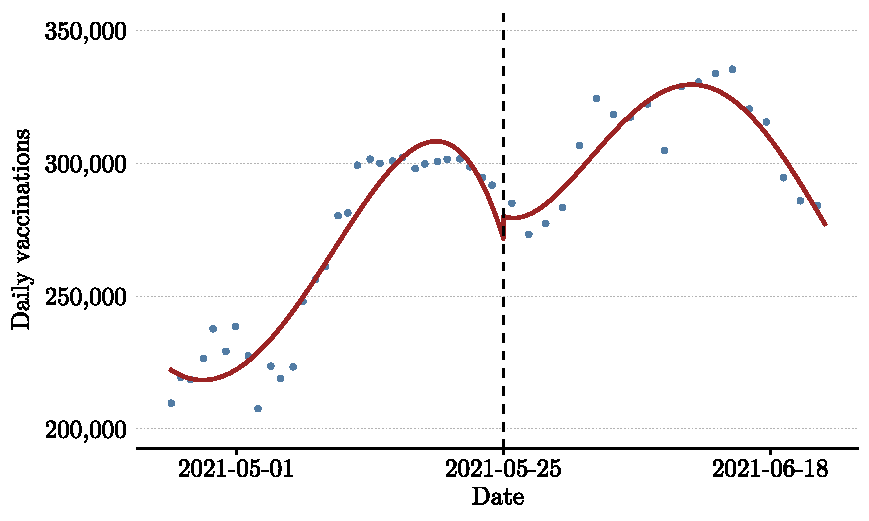
\includegraphics{bachelor_thesis_files/figure-latex/unnamed-chunk-2-1} \end{center}
\end{figure}

\vspace{-1.2cm}
\begin{table}[! htbp]\centering \caption[Results of regression discontinuity analysis of daily vaccinations in Poland]{Regression results of regression discontinuity analysis of daily vaccinations.}
\bigskip
\label{table:weightssynth}
\begin{threeparttable}
\begin{tabular}{c c c}
\toprule
 & (1) & (2)\\
 & Uniform & Triangular\\
 & Kernel & Kernel\\ \midrule
Bandwidth & 11.014 & 12.512\\
Estimate & 7236.471 & 4567.651\\
Std. Error & 16199.275 & 16579.766\\
z & 0.447 & 0.275\\
P>|z| & 0.655 & 0.783\\
95\% CI & [-24513.525, 38986.467] & [-27928.093, 37063.395]\\
\bottomrule\addlinespace[1ex]
\end{tabular}
\end{threeparttable}
\label{table2}
\end{table}

Figure 3.1 presents the results of the analysis (uniform kernel). By
comparing the regressions before and after the cutoff, a slight increase
in daily vaccinations around the time of announcement can be observed.
With corresponding regression discontinuity estimates (\(\hat{\beta}\))
of 7,236.5 (uniform kernel) and 4,567.7 (triangular kernel) additional
daily vaccinations, this effect can however not be regarded as
significant (in both specifications), as the respective
\textit{p}-values in Table 4.1 show. During the examined time frame,
daily vaccinations were close to their all-time high. Nonetheless, the
Polish government felt the need to incentivize their citizens with a
lottery.

\begin{figure}[h]
\caption[Synthetic control analysis of the Polish lottery (share of the fully vaccinated)]{The synthetic control analysis of the share of the population fully vaccinated against COVID-19 shows a decoupling between Poland and Synthetic Poland, as well as a subsequent narrowing of the gap.}

\begin{center}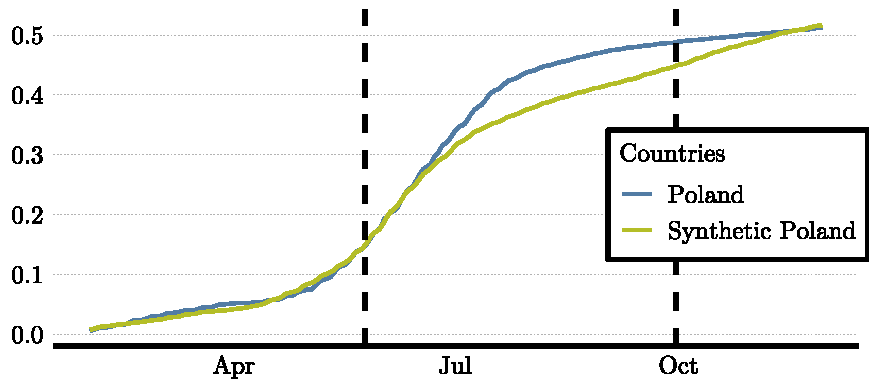
\includegraphics{bachelor_thesis_files/figure-latex/unnamed-chunk-3-1} \end{center}



\begin{center}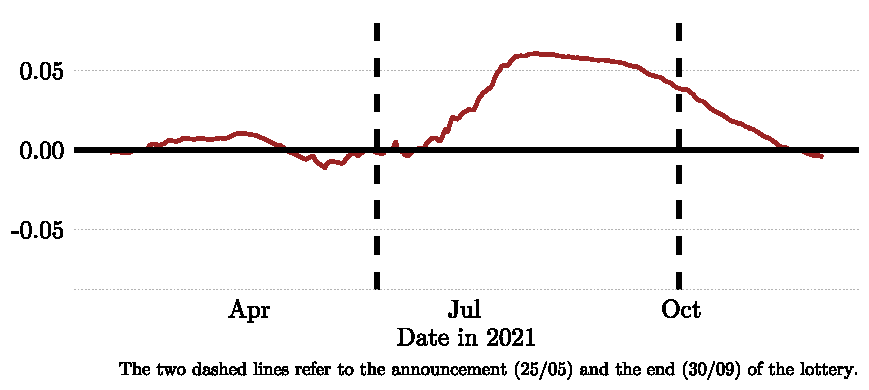
\includegraphics{bachelor_thesis_files/figure-latex/unnamed-chunk-3-2} \end{center}
\end{figure}

\vspace{-0.5cm}

Next, the synthetic control method was applied to investigate the impact
on vaccination rates, as described in Section 3.4. Figure 4.2 plots the
vaccination rate (fully vaccinated) for both Poland and Synthetic
Poland. The pre-treatment fit of the synthetic control unit was not
perfect, but relatively good, with a maximum variation of around one
percentage point from actual Poland. Following a short lag after the
intervention, a slow decoupling between Poland and its synthetic control
unit can be observed. This difference continues to increase to a maximum
of around five percentage points, around the end of July/beginning of
August. As time progresses, the gap tends to decrease again and by the
end of September (end of the lottery), the vaccination rates of Poland
and Synthetic Poland were nearly back to the same level, with a
remaining difference of around one percentage point.

\begin{figure}[h]
\caption[Placebo plot of Poland and donor pool]{Estimated differences between actual and synthetic control units do not suggest a signficant effect. The synthetic control units of the donor pool countries are placebos (constructed as if there was a treatment).}

\begin{center}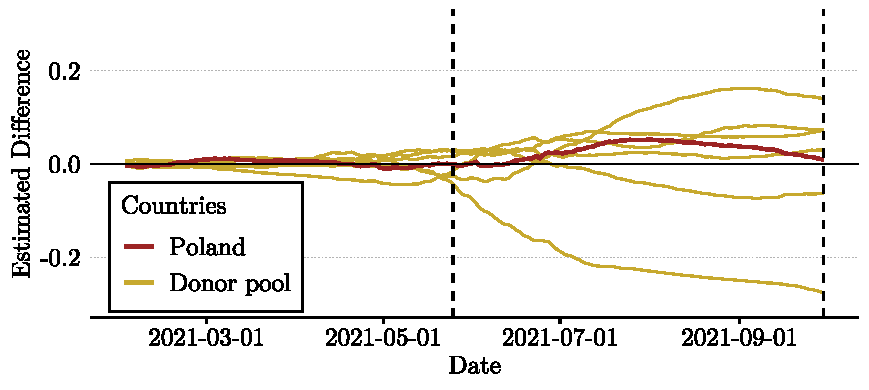
\includegraphics{bachelor_thesis_files/figure-latex/unnamed-chunk-4-1} \end{center}
\end{figure}

\vspace{-0.2cm}

In order to answer whether the estimated effect of one percentage points
was statistically significant, the permutation based inference
techniques, discussed in Section 3.3, were employed. Figure 4.3 presents
the placebo study. As observable, the magnitude of the effect for Poland
was not comparably high. In fact, the effect for Poland was one of the
least extreme of all of the selected units. This finding was also
confirmed quantitatively. Using the discussed procedure, a
\textit{p}-value of 0.571 was obtained, meaning that the observed effect
was not statistically significant. Therefore, the hypothesis that the
lottery had no effect on vaccination rates cannot be rejected.

\subsection*{Robustness checks}

\begin{figure}[h]
\caption[Robustness check: Time of intervention]{Adjustments in the time of intervention change the direction of the estimated effect.}

\begin{center}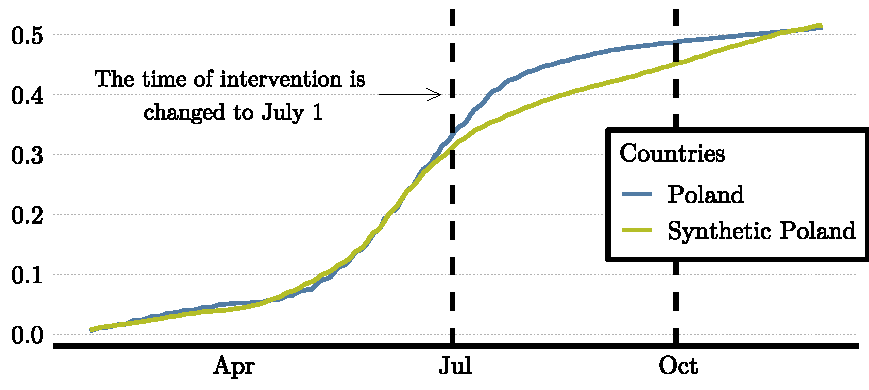
\includegraphics{bachelor_thesis_files/figure-latex/unnamed-chunk-5-1} \end{center}



\begin{center}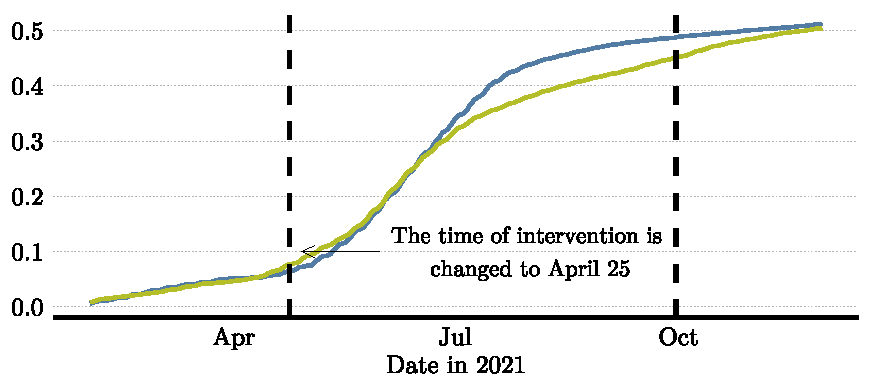
\includegraphics{bachelor_thesis_files/figure-latex/unnamed-chunk-5-2} \end{center}
\end{figure}

Next, the robustness of the synthetic control of the share of the fully
vaccinated was assessed. Firstly, the time of the intervention was
changed. As discussed earlier, there were two plausible intervention
points: The announcement and the start of the lottery, with the
announcement as the preferred option. In order to inspect the robustness
of the synthetic control unit, July 1, the start of the lottery was used
as the intervention time. As the upper panel of Figure 4.4 shows,
changing the time of intervention from May 25 to July 1, 2021 had a
considerable effect on the synthetic control unit (largest absolute
change of a single weight: 0.631 (Slovenia)), but although the direction
of the estimated effect changed, this effect can also not be regarded as
significant (\textit{p}-value: 0.714).

A second way of changing the time of intervention is backdating, meaning
that the effect is estimated using an arbitrary earlier intervention
time. A new synthetic control unit was therefore constructed, with a
``fictional'' intervention time one month (April 25, 2021) prior to the
actual announcement. As observable in the lower panel of Figure 4.4, the
changes are clearly visible (largest absolute change of a single weight:
0.84 (Estonia)), but the new synthetic control was still able to track
the path of actual Poland relatively well. Similar to the first change
of intervention time, the estimated effect was also not significant
(\textit{p}-value: 0.714).

\begin{figure}[h]
\caption[Robustness check: Leave-one-out analysis]{Leave-one-out analysis with respect to predictors (upper panel) and donor pool countries (lower panel) generates large discrepancies in the estimated effect.}

\begin{center}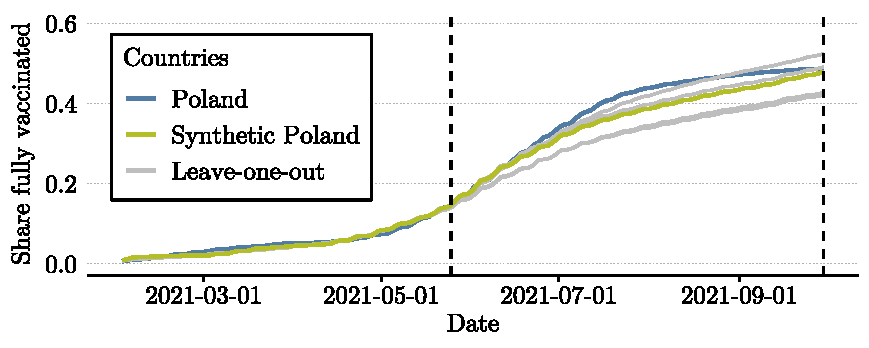
\includegraphics{bachelor_thesis_files/figure-latex/unnamed-chunk-6-1} \end{center}



\begin{center}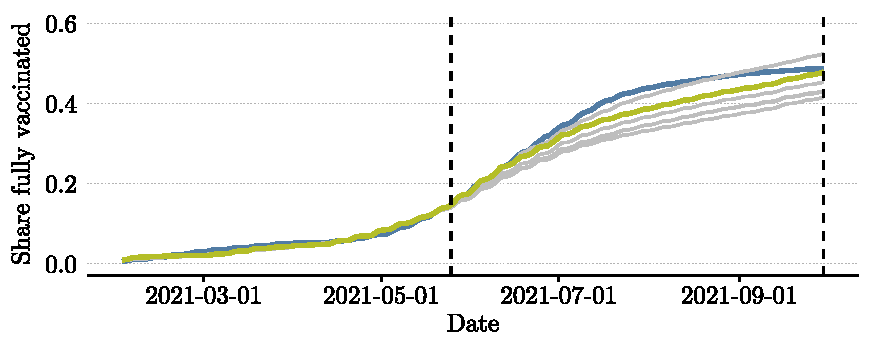
\includegraphics{bachelor_thesis_files/figure-latex/unnamed-chunk-6-2} \end{center}
\end{figure}

Another possible robustness check is to leave out certain predictors or
countries. Figure 4.5 presents the result of a leave-one-out analysis of
synthetic Poland, leaving out all of the predictors once, while keeping
the others in, repeating the same with respect to donor pool countries
(solving the constrained minimization with only five donor pool
countries). This robustness check also showed considerable effects on
the synthetic control unit. In both the upper and the lower panel of the
figure, large discrepancies (around ten percentage points) in the
estimated effect arose.

A synthetic control analysis of the share of the population with at
least one dose of any COVID-19 vaccination was also carried out. While
the results showed differing patterns compared to the presented analysis
of the fully vaccinated (possibly suggesting a negative impact of the
lottery of close to nine percentage points), there also seemed to be no
statistically significant effect, with a \textit{p}-value of 0.143. The
corresponding Figure A.1 can be found in the appendix.

\chapter{Discussion}

Contrary to \textcite{kuznetsova_effectiveness_2022}, the results of a
regression discontinuity design, applied to daily vaccinations in
Poland, do not suggest an increase in daily vaccinations as a result of
the lottery. The most likely reason for this discrepancy is that the
study by \textcite{kuznetsova_effectiveness_2022} used the start of the
lottery (July 1, 2023) as the time of intervention. In contrast, the
presented analysis employed the day of announcement as the cutoff value.
In principle, both dates seem appropriate, but, as outlined, because the
date of vaccination did not matter for entering the lottery, the day of
announcement was chosen as the preferred option.

The results of the synthetic control analysis showed that there was no
statistically significant change in the vaccination rate of the fully
vaccinated. One possible interpretation of the results pictured in
Figure 4.2 might be that people who would have gotten vaccinated anyways
decided to do this earlier, to take advantage of the lottery. This could
explain the temporarily larger gap (decoupling between the two units and
subsequent narrowing of the gap) between Poland and Synthetic Poland.
So, while the lottery was not successful in getting more people
vaccinated, it could have possibly induced people to get vaccinated
earlier.

The robustness checks indicated that the main finding (no significant
effect) is robust with respect to the time of intervention, thereby
confirming that this application of the synthetic control method did not
suffer from an anticipation effect. But, since considerable differences
in the shape of the synthetic control unit arose, the overall pattern
(beyond the main result of no significant effect) cannot be considered
as robust.

When performing the leave-one-out analysis, large discrepancies (ten
percentage points) in the estimated effect were observable, also with
respect to its direction. Given the relatively low number of donor pool
countries and predictor variables, this result is not particularly
surprising and underlines the importance of the specifications of a
synthetic control analysis. Although making small adjustments to the
specifications of the analysis might seem trivial, it potentially
changes the overall interpretation of the result quite considerably
(direction of the effect).

Lastly, the analysis of the share of the population with at least one
dose of any COVID vaccine generated a very different pattern (large
negative effect) compared to the main analysis, while also confirming
the main result (no significant effect). This additionally showed that,
generally, the presented synthetic control estimation is not very
robust.

There are several limitations of this application of the synthetic
control method, restricting the internal validity of the results and the
derived interpretation.

Firstly, the composition of donor pool countries was not ideal, with a
low number of countries as well as considerable differences between the
control units. As a consequence, the number of possible combinations of
the weights was limited, e.g.~compared to a synthetic control analysis
of the lottery in Ohio (for example \textcite{barber_conditional_2022}),
where all other US States (minus states that implemented similar
policies) could in principle be selected for the donor pool. The low
number of donor pool countries was also problematic for the inference
procedure, since it was difficult to obtain a good fit of the synthetic
control unit for six different countries: One of the placebo synthetic
controls estimated a negative effect of more than 20 percentage points
for one of the donor pool countries. This seems to be unrealistic and
not consistent with the size of the estimated effects of other vaccine
lotteries (e.g.~\cite{robertson_are_2021};
\cite{acharya_implementation_2021}; \cite{fuller_assessing_2022}).
Therefore, not only the interpretation but also the main result itself
(no significant effect), should be treated with caution, because the
size of the estimated effect of Poland would have to be very large to be
extreme compared to the placebo synthetic controls.

Ohio is also a valuable example regarding the similarity between the
treated unit and the donor pool units. Other US states are often
relatively similar to Ohio, both in terms of general characteristics as
well as vaccination rates \parencite{mathieu_global_2021}. Although the
donor pool countries in this thesis were selected to be not too
different compared to
Poland\footnote{See Table 3.1 for a comparison between Poland and the average of the donor pool.},
cross-country differences are expected to be larger than cross-state
differences. Overall, the low number of donor pool countries and a
restricted similarity between Poland and the donor pool limit the
validity of the synthetic control analysis significantly.

Secondly, the effect of the vaccine lottery might have been too small to
be relevant for a synthetic control analysis. The effect on vaccination
rates that has been estimated for similar lotteries is often relatively
small (e.g.~\textcite{barber_conditional_2022}: 1.5\%). Poland's lottery
offered more prizes, but a lower main prize than some lotteries in North
America. It might therefore be conceivable that the effect of the given
policy in Poland was too small for a valid synthetic control analysis,
since the impact of the intervention might not have been distinguishable
from other relatively small shocks to the vaccination rate (e.g.~a
public marketing campaign to get vaccinated).

Another possible limitation of this analysis are the imputed values. As
explained in Section 3.2, some countries in the donor pool did not
report their vaccination rates on all days, including the country of
interest (Poland). Although the results of the interpolation looked
reasonable for all of the donor pool countries, this might still have
had a negative effect on the credibility of the presented synthetic
control, since undesired changes in the chosen weights of the synthetic
control unit could have been caused.

At the same time, there are also requirements of the synthetic control
method which this application should have fulfilled. Firstly, no signs
of an anticipation effect were observed, as discussed. Secondly, the
possibility of spillover effects: There is no plausible argument for the
presence of spillover effects. Since countries who adopted similar
incentive policies were removed, no country in the donor pool used the
Polish lottery as an example for similar action. Lastly, the number of
pre-intervention observations of the outcome variable does not represent
a problem. The outcome variable was taken into account from February 1,
2021 until the day prior to the announcement (May 24, 2021). Since daily
data was employed, a total of 113 pre-intervention observations of the
outcome variable were used, meaning that the number of predictors in the
optimization was high (all 113 pre-intervention observations plus the
additional predictor variables).

To improve the internal validity, two additional predictor variables
were considered, but ultimately not selected. One of these was a
``political variable'', since differences in vaccine uptake exist across
party preferences. While this problem might be the most well-known in
the US \parencite{ruiz_predictors_2021}, it is also believed to be a
relevant predictor of vaccine uptake (even before COVID-19) in Europe
(\cite{schernhammer_correlates_2022}; \cite{kennedy_populist_2019}).
But, when using other European countries as a donor pool, it is
difficult to compare political beliefs across countries, mainly because
of large differences in party ideologies. One could use the vote share
for parties along the groups in the European Parliament, but this is not
unproblematic: There are large differences between parties within
certain
groups\footnote{For example, the Renew Europe group in the EP consists of liberal parties in a very broad sense, including both left of centre liberal parties and liberal-conservative parties.}
and the relatively wide political landscape in Europe (e.g.~compared to
a two party system) may make differences in attitudes toward the
COVID-19 vaccine hard to compare.

Another predictor which was considered is trust in government, with the
data also available from the Wellcome Global Monitor. Trust in
government is potentially volatile. For example, when an unpopular
government is replaced by a new government, this might increase the
trust into the public sector dramatically in a very short time span. The
problem of high volatility should have been especially pronounced in a
time of crisis like the COVID-19 pandemic, where large variations in
infection rates could have lead to quick changes in public opinion.
While there may also exist deep-rooted cross-country differences in
trust in government (e.g.~possibly higher distrust in former soviet
influenced countries compared to western countries
\parencite{costa-font_institutional_2023}), the possible presence of the
described volatility meant that the variable trust in government was not
selected.

To summarize, it is important to note that the causal interpretation of
the given results should not be overstated, because of the outlined
threats to internal validity as well as a restricted robustness. As
shown in Section 2.1, even when investigating the same lottery (Ohio)
using the synthetic control method, studies showed differing results,
since the specifications of the synthetic control analysis can have
considerable consequences on the estimated effect. Regarding the
external validity, this thesis presented only one case study of vaccine
lotteries. While the results do not suggest a significant effect of the
lottery on the vaccination rate, the applicability of these results on
(at first glance) comparable policies is limited, mainly because of
differences in the design of lotteries, initial vaccination rates as
well as other country-specific predictors.

\chapter{Conclusion}

What are the effects of vaccine lotteries on the share of the population
vaccinated against COVID-19? The existing literature suggests that
vaccine lotteries might have increased vaccination rates, for example in
Ohio, where several studies found positive effects on vaccine uptake
(\cite{mallow_covid-19_2022}; \cite{brehm_ohio_2022};
\cite{barber_conditional_2022}; \cite{sehgal_impact_2021}). However, the
majority of the work on vaccine lotteries has so far focused on the
evaluation of state vaccine lotteries in the US.

This thesis provided an in-depth evaluation of a vaccine lottery in
Europe, adding an additional case study on the effectiveness of such
programs to the existing literature. Specifically, a vaccine lottery
implemented in Poland, from July 1, 2021 to September 30, 2021, was
empirically examined. The lottery consisted of cash and non-cash prizes,
totaling to around 140 million zł. To estimate the effect of this
program on vaccination rates, the synthetic control method was selected.
Synthetic Poland was constructed out of a donor pool of six other
Eastern European countries.

The results of the main analysis showed no signs of a statistically
significant (\textit{p}-value: 0.571) increase in the vaccination rate
(fully vaccinated) compared to the hypothetical scenario without the
lottery. Additionally, a regression discontinuity analysis did not find
a significant effect of the lottery on daily vaccinations around the day
of announcement. While the synthetic control estimation did not show to
be very robust, it was observed that vaccination rates (fully
vaccinated) increased in the short-run, thereby possibly suggesting that
people who would have gotten vaccinated anyways may have chosen to do
this earlier, as a result of the lottery.

\AtEndDocument{\pagebreak
\begin{appendices}

\addcontentsline{toc}{chapter}{Appendix}


GitHub repository: \url{https://github.com/benediktstelter/bachelor_thesis}

\noindent All of the data for the additional predictor variables as well as the R scripts used to analyse the data can be found in the folder "scripts\_data".

\begin{figure}[h]
\caption[]{The analysis of the share of the population with at least one dose of any COVID vaccination shows different patterns, but also does not suggest a significant effect.}

\begin{center}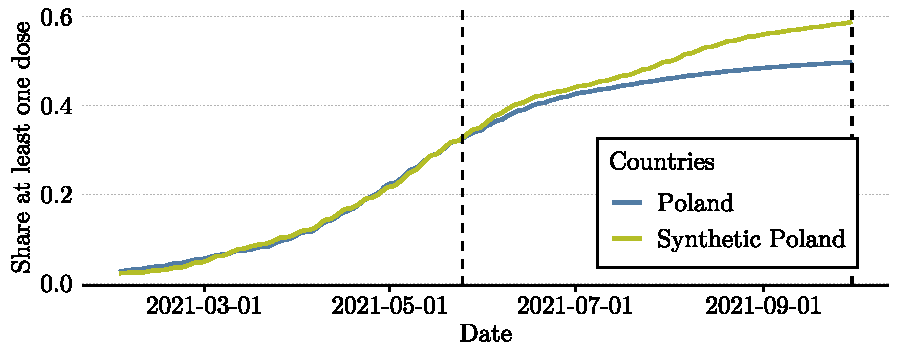
\includegraphics{bachelor_thesis_files/figure-latex/unnamed-chunk-8-1} \end{center}



\begin{center}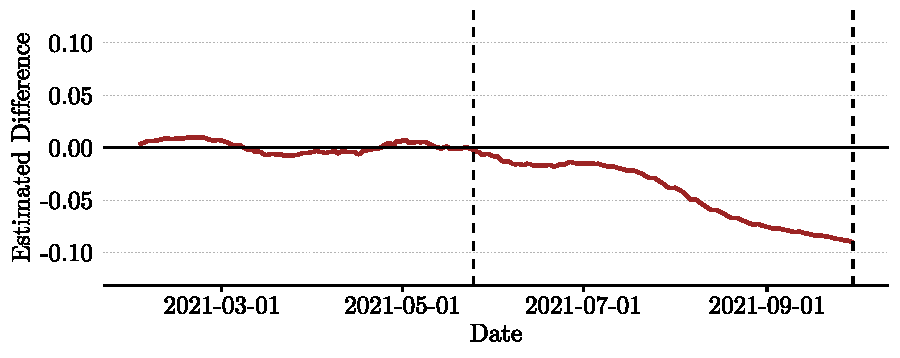
\includegraphics{bachelor_thesis_files/figure-latex/unnamed-chunk-8-2} \end{center}
\end{figure}


\begin{figure}[h]
\caption[]{Placebo Plot: Share with at least one dose.}

\begin{center}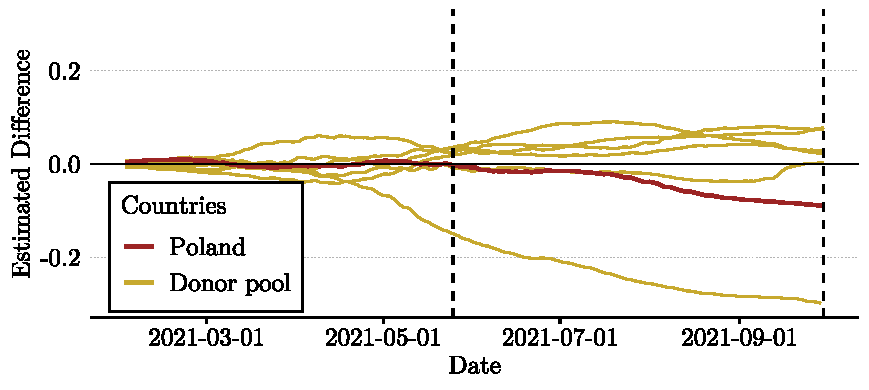
\includegraphics{bachelor_thesis_files/figure-latex/unnamed-chunk-9-1} \end{center}
\end{figure}


\end{appendices}

\chapter*{Affidavit}
\addcontentsline{toc}{chapter}{Affidavit}

\thispagestyle{empty}



I affirm that this Bachelor thesis was written by myself without any unauthorized third-party support. All used references and resources are clearly indicated. All quotes and citations are properly referenced. This thesis was never presented in the past in the same or similar form to any examination board. 

\noindent I agree that my thesis may be subject to electronic plagiarism check. For this purpose an anonymous copy may be distributed and uploaded to
servers within and outside the University of Mannheim.

\vspace{2\baselineskip}

\noindent Ich versichere, dass ich die vorliegende Arbeit ohne Hilfe Dritter und ohne Benutzung anderer
als der angegebenen Quellen und Hilfsmittel angefertigt und die den benutzten Quellen
wörtlich oder inhaltlich entnommenen Stellen als solche kenntlich gemacht habe. Diese Arbeit
hat in gleicher oder ähnlicher Form noch keiner Prüfungsbehörde vorgelegen.

\noindent Ich bin damit einverstanden, dass meine Arbeit zum Zwecke eines Plagiatsabgleichs in
elektronischer Form anonymisiert versendet und gespeichert werden kann.

\vspace{4\baselineskip}
\begin{center}
\parbox{.8\textwidth}{Mannheim, 17/03/2023 \hfill Benedikt Stelter}
\end{center}


}


 
\backmatter


 
\renewcommand\refname{References}
\printbibliography[title=References]


\newpage
\newenvironment{appendices}
    {\chapter*{Appendix}
\renewcommand{\thetable}{A.\arabic{table}}
\renewcommand{\thefigure}{A.\arabic{figure}}
\setcounter{table}{0}
\setcounter{figure}{0}
    }






 
\end{document}
